\documentclass[../main.tex]{subfiles}

\begin{document}
\chapter{ASG Language}
ASG is a graphical \define{specification language} for distributed real-time systems and belongs to the family of \define{hierarchical state languages} such as \textit{\define{STATECHARTS}}, \textit{TTM} (Timed Transition Models) and \textit{\define{MODECHARTS}}.
All these languages have been introduced progressively from 1987.
They allow to describe the behavior of systems and have enhanced the expressiveness of state machines by introduction of time, hierarchies and parallelism.
This avoids the explosion of the number of states and allows reasoning at different abstraction levels.
It was intended to be readable by non computer-scientists, in order to be able to verify that what is specified is actually what the client wanted.
\\\\
ASG, which was developed by \define{UCLouvain}, has some specific characteristics.
\begin{itemize}
	\item It takes into account the impossibility to detect instantaneously a state change in a distributed system if it happens remotely (\define{transmission delay}).
	\item It offers more restrictive rules on the destination state of a transition, e.g. it is not allowed to go to any other state that the initial sub-state of a state refined in sub-states if not coming from another sub-state of the same refinement.
    This allows to reason at a given hierarchical level without considering what happens at lower levels.
    Consequently this promotes a top-down design, by refining states into sub-states when appropriate.
\end{itemize}

\section{Language Elements}
An ASG diagram consists of \textbf{states} and \textbf{transitions}. Crossing a \define{transition} is instantaneous: the system is thus always in a state.
\begin{figure}[H]
    \centering
    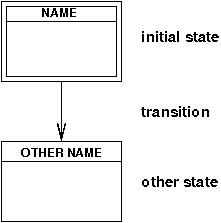
\includegraphics[width=0.25\textwidth]{asg1.jpg}
    \caption{ASG States and Transitions}
    \label{asg1}
\end{figure}

\subsection{States}
Each state has a name and some \textbf{time-related state properties:}
\begin{itemize}
	\item \definebf{MINVT}: The \textbf{minimum visit time} is the minimum time the system remains in the state.
	\item \definebf{Time-Out}: A time-out counter is started when the state is entered. When this time-out duration has elapsed, a boolean variable \texttt{state\_name.timout} becomes true if the system is still in that state.
\end{itemize}

A state has an \definebf{action} which is executed when the state is entered.
When the action is finished, the system might choose to wait in the current state.
Executing the action takes some time and can be seen as happening in parallel with the system staying in the state.
An action consists of 3 steps:
\begin{enumerate}
	\item Read the necessary data
	\item Process the data
	\item Write the results atomically
\end{enumerate}
An action has one property: its \definebf{deadline}, the maximum amount of time the action is allowed to take.
The deadline is a \definebf{declarative temporal specification}: the system should be fast enough to respect that constraint.
However, since the system assumes that deadlines are always respected, it's ignored by the system and a constraint for the implementer.
On the other hand, \textbf{MINVT} and \textbf{time-outs} are elements that the system's behavior has to take into account.
\\\\
Further properties of a state include a \definebf{rendez-vous label}.
This is used to synchronize parallel behavior.
Another property is a list of \textbf{resources} that  prevents parallel behavior to reach incompatible states.

\subsection{Transitions}
\begin{defn}
An \textbf{event is detected} when the system learns the following in the origin state:
\begin{center}
The system is in the origin state of the transition \textbf{and} the condition associated with the transition is true.
\end{center}
\end{defn}

\begin{figure}[H]
    \centering
    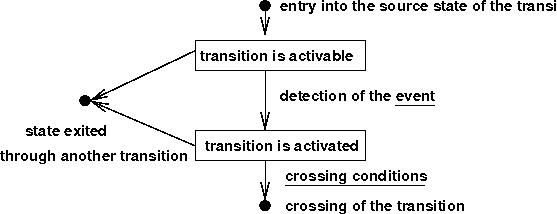
\includegraphics[width=0.5\textwidth]{asg2.jpg}
    \caption{ASG Transitions}
    \label{asg2}
\end{figure}

The condition is any boolean expression, based on environment variables or booleans indicating a \textit{rendez-vous} or \textit{time-out}.
In a distributed system some time is needed in order to detect a state change of a remote variable.
To avoid \definebf{hidden delays} the system works with local state changes and the local perception of the remote state.
\begin{figure}[H]
    \centering
    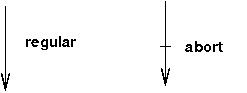
\includegraphics[width=0.3\textwidth]{asg3.jpg}
    \caption{ASG Regular and Abort Transition}
    \label{asg3}
\end{figure}
When a \define{transition event} is detected, the action is not necessarily finished, the time spent in the state is not necessarily larger that MINVT and resources required to enter the destination state are not necessarily available. This gives cause to two families of transitions. The \definebf{crossing condition} depends on the transition family.
\begin{enumerate}
	\item  The crossing conditions of \definebf{regular transitions} (figure \ref{asg3}, left) are the following:
	\begin{itemize}
		\item The action is finished.
		\item The time spent in the state $/geq$ MINVT.
		\item All resources are available.
		\item No transition with a higher priority is active.
	\end{itemize}
	\item The crossing conditions of \definebf{abort transitions} (figure \ref{asg3}, right) is limited to the absence of a higher priority transition allowed to leave its state.
\end{enumerate}

\section{Diagram Structure}
As with similar languages, there are two ways to structure the diagrams: \definebf{parallelism} and \definebf{hierarchy}.

\subsection{Hierarchy}
\begin{figure}[H]
    \centering
    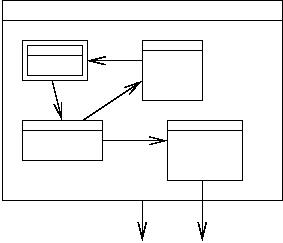
\includegraphics[width=0.4\textwidth]{asg4.jpg}
    \caption{ASG Hierarchy}
    \label{asg4}
\end{figure}
Any state may be refined in mutually exclusive \define{sub-states}.
Any such sub-state is a state that may itself be refined.
The system is both in the outer state as well as in the sub-state.
Actions may be associated with the outer state and with each sub-state, at any level, including the initial sub-states.
Actions attached to the outer state and to the initial sub-state start simultaneously and are performed in parallel.
\begin{figure}[H]
    \centering
    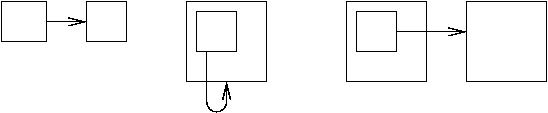
\includegraphics[width=0.6\textwidth]{asg5.jpg}
    \caption{ASG Hierarchic State Leaving}
    \label{asg5}
\end{figure}
A transition leaving a state may only end in a \define{sibling state} (a state belonging to the same refinement), an \define{ancestor state} (a state enclosing the current state) or the sibling of an ancestor.
A state can be exited trough a transition leaving this state itself, leaving a state enclosing this state or leaving a state included in this state.
\begin{exmp}
State A could be exited trough transitions $i$, $j$ and $k$.
\begin{figure}[H]
    \centering
    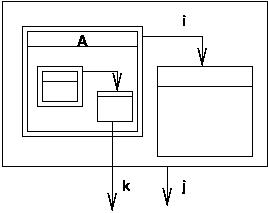
\includegraphics[width=0.4\textwidth]{asg6.jpg}
    \caption{ASG Example Leaving State}
    \label{asg6}
\end{figure}
\end{exmp}
Conditions of a transition must be satisfied for all the states that would be exited.
(The system might have to wait for several actions to be completed and several MINVT to be elapsed)

\subsection{Parallelism}
In ASG, parallelism is always explicit by refining the state into several parallel components. Note that exiting a state through 2 transition at a time is not allowed in ASG.

\begin{figure}[H]
    \centering
    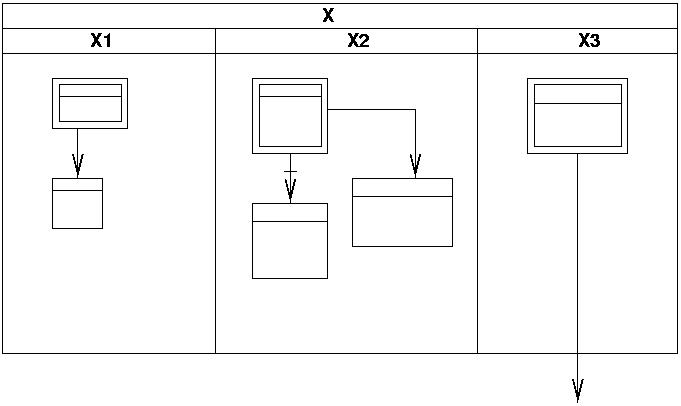
\includegraphics[width=0.6\textwidth]{asg7.jpg}
    \caption{ASG Parallelism}
    \label{asg6}
\end{figure}
When a state, refined in parallel components is entered, the initial sub-states of all the parallel components are entered at the same time.
If the refined state is exited from one of the parallel components, all the parallel components are terminated.
(Exiting the refined state may be through a regular or trough an abort transition)

\section{ASG Components}

\subsection{Transition Priority Rules}
One of the \definebf{crossability conditions} of a transition is to have the highest priority of all transitions conflicting \index{Conflicting Transitions} with it. Transitions are called conflicting when they are activated and the highest state (in hierarchy) exiting is the same, or an ancestor, of the other state.
\\\\
\define{Priority Rules}:
\begin{enumerate}
	\item An abort transition has a higher priority that a regular transition. If the state can be exited through several abort transition, one is selected according to the following rules.
	\item If the outermost state exited by an abort transition encloses that of another abort transition, the former will have a higher priority.
	\item Numbered transitions with a lower number have a higher priority. Unnumbered transitions have the lowest priority.
	\item A transition activated before another has a higher priority than the latter.
	\item If none of the above rules apply, a transition is selected at random.
\end{enumerate}

\subsection{The Rendez-Vous}
Rendez-vous labels are associated with states.
A rendez-vous happens when all the parallel components active and concerned by the same rendez-vous label are in a state labeled with that same rendez-vous.
An ]\define{active parallel component} means that the system is in one of its states.
A state is \define{concerned} with a rendez-vous label if at least one of its states is labeled with it.
\\\\
A rendez-vous allows many types of synchronizations between parallel components.
The simplest is to \define{trigger} a transition in a parallel component when a job is finished in another one.
Generally a label will be assigned to the state following the one with the action.
If necessary, a empty state (without an action) can be added for this purpose.
Another use of the rendez vous is allowing a parallel decomposition to exit in a disciplined way.
\begin{figure}[H]
    \centering
    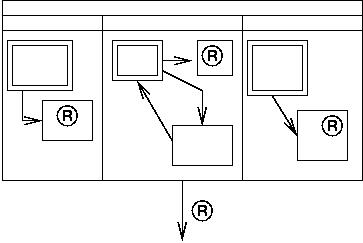
\includegraphics[width=0.6\textwidth]{asg8.jpg}
    \caption{ASG Rendez-Vous}
    \label{asg8}
\end{figure}

Nothing guarantees that two transitions (in different parallel components) will transition simultaneously, even if their event has the same rendez-vous point.
This is because transition conditions could be delayed and if the system is distributed, the event will not necessarily be perceived simultaneously everywhere.
\\\\
In a distributed system, the detection of a rendez-vous is not necessarily immediate, but all rendez-vous will be detected, on condition that the time intervals in which the rendez-vous states are occupied overlap at least in part.
\begin{figure}[H]
    \centering
    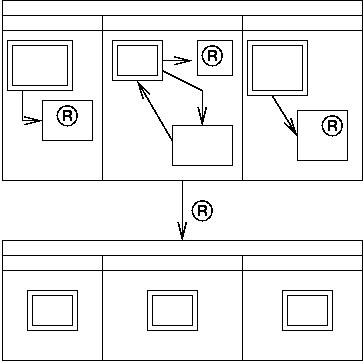
\includegraphics[width=0.6\textwidth]{asg9.jpg}
    \caption{ASG Rendez-Vous}
    \label{asg9}
\end{figure}

\subsection{Resources}
\define{Resources} allow the system to get temporarily \define{exclusive access} to a shared component. When resources are needed in u sub-state of some parallel component, the sub-states are labeled with their required resource.


\begin{figure}[H]
    \centering
    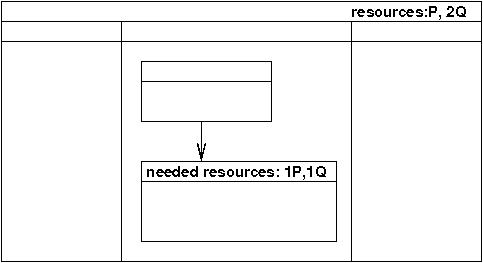
\includegraphics[width=0.6\textwidth]{asg10.jpg}
    \caption{ASG Resources}
    \label{asg10}
\end{figure}
A parallel component must have obtained the \define{exclusive right} to use of all the resources necessary in the next state before being allowed to transition to this state.

Resources are requested by a parallel component as soon as the transition to enter this state is activated.
Resources are held until either a higher priority transition (through which the source state could exit) is activated or until the state that needed the resource is exited.
\\
Obtaining a requested resources may take some time.
The system might have to wait until the resources are freed by the previous user, especially when several resources are needed to enter a state.
In order to avoid \define{deadlocks} when gathering resources needed to cross a transition, a parallel component must always obtain resources in the reverse order of their declaration

\begin{exmp}
The left component will cause a deadlock if it does not respect the last rule.
\begin{figure}[H]
    \centering
    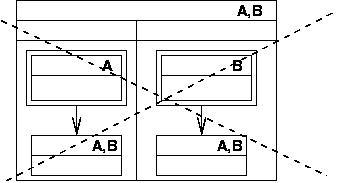
\includegraphics[width=0.5\textwidth]{asg11.jpg}
    \caption{Deadlock}
    \label{asg11}
\end{figure}
\end{exmp}
The aim of resources is to express \define{mutual exclusion} between states of different parallel components.
\begin{exmp}
Creating starvation situations with resources, making some states unaccessible is easy, as illustrated below.
\begin{figure}[H]
    \centering
    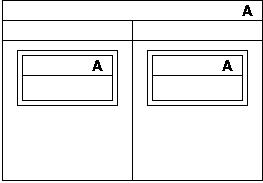
\includegraphics[width=0.4\textwidth]{asg12.jpg}
    \caption{Deadlock}
    \label{asg12}
\end{figure}
However, a \define{static analysis} of the diagram allows identifying the sets of \define{mutually exclusive states} and those that are not accessible.
\end{exmp}

\section{Examples}
\begin{exmp}
An elevator will only change direction if there are no more requests left in the current direction. The states \textit{stopped}, \textit{doors opening} and \textit{doors opened} all have a \textbf{MINVT} to give the doors time to open and let people leave the elevator. The \textit{open} state has a time-out after which the doors are closed. Consider the following activation conditions:
\begin{enumerate}
	\item detection\_door\_completely\_open
	\item movement\_requested or open.timeout or close\_doors\_button\_pressed
	\item presence\_detected\_in\_door\_opening
	\item detection\_door\_fully\_closed
	\item always true
	\item movement\_request\_in\_current\_direction
	\item arrival\_at\_destination\_floor or arrival\_at\_calling\_floor\_in\_current\_direction or \\ (no\_other\_destination\_ in\_current\_direction and arrival\_at\_calling\_floor\_in\_other\_direction)
	\item movement requested\_in\_other\_direction or called\_from\_other\_direction
	\item true
\end{enumerate}
In order to be complete, one should add parallel components memorizing movement requests and a component to remove the request at each floor when the destination is reached.
\end{exmp}

\begin{exmp}
A sluice has two doors $P_1$ and $P_2$ and 5 sensors $X,Y,Z,V,W$ to detect the presence of a ship. Sensors  $X, Y$ and $Z$ are located in front of the doors and inside the sluice. Sensors $V$ and $W$ are located in such a way that they can detect the presence of the ship when passing the doors.

\begin{figure}[H]
    \centering
    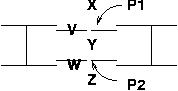
\includegraphics[width=0.3\textwidth]{asg13.jpg}
    \caption{Sluice}
    \label{asg13}
\end{figure}
Only one of the sluice's doors may be opened at a time. Outgoing traffic (from X to Z) always has priority.
\\\\
\textbf{Sequential Solution}\\
The sequential solution simply expresses that there are two sequences that are allowed.
\begin{figure}[H]
    \centering
    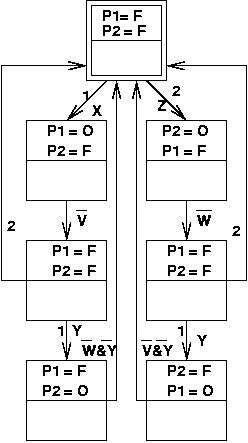
\includegraphics[width=0.5\textwidth]{asg14.jpg}
    \caption{Sequential Solution}
    \label{asg14}
\end{figure}
To be complete, each state should be refined in two sub-states: door sliding and door in position
\\\\
\textbf{Parallel Solution} \\
A resource is used to prevent the two doors to open simultaneously.
\begin{figure}[H]
    \centering
    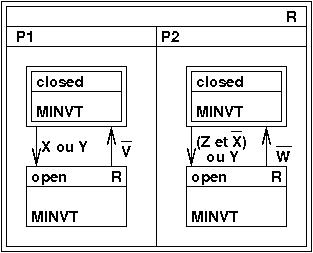
\includegraphics[width=0.5\textwidth]{asg15.jpg}
    \caption{Parallel Solution}
    \label{asg15}
\end{figure}
The purpose of the MINVT in the \textit{open} states is to allow ships to enter or exit the sluice. Otherwise, the doors would just open and close without letting anybody in.
\end{exmp}


\end{document}